\chapter{Opis interfejsu uzytkownika}

\section*{Panel logowania}
\begin{figure}[H]
\centering
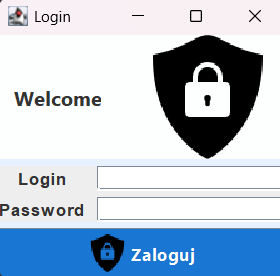
\includegraphics[width=0.4\textwidth]{figures/workApl/login_panel.png}
\caption{Panel logowania do systemu}
\label{fig:login_panel}
\end{figure}

Panel logowania umożliwia autoryzację użytkownika przed uzyskaniem dostępu do głównego interfejsu systemu. Użytkownik wprowadza dane w pola \texttt{Login} i \texttt{Password}, a następnie klika przycisk \textbf{Zaloguj}. Przy nieprawidłowych danych wyświetlany jest komunikat błędu.

\section*{Główny panel sekretariatu}
\begin{figure}[H]
\centering
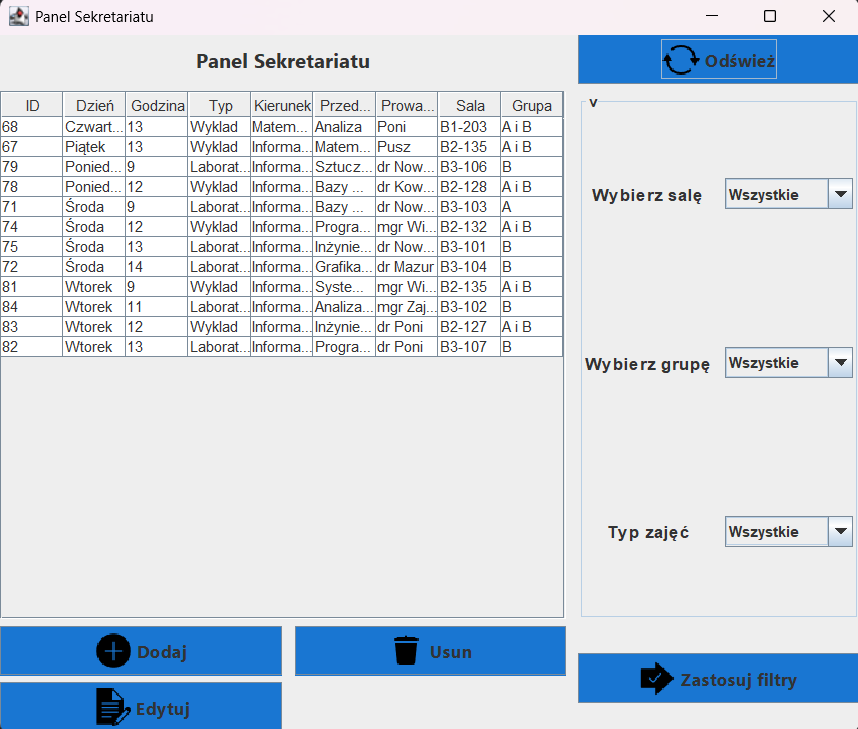
\includegraphics[width=\textwidth]{figures/workApl/mainpanel.png}
\caption{Główny panel sekretariatu z listą zajęć i filtrowaniem}
\label{fig:mainpanel}
\end{figure}

Główny panel aplikacji wyświetla listę wszystkich zajęć w formie tabeli. Użytkownik może:
\begin{itemize}
    \item \textbf{Dodawać zajęcia} – klikając przycisk \textbf{Dodaj},
    \item \textbf{Edytować istniejące zajęcia} – po zaznaczeniu wiersza i kliknięciu \textbf{Edytuj},
    \item \textbf{Usuwać zajęcia} – klikając przycisk \textbf{Usuń},
    \item \textbf{Filtrować dane} – za pomocą rozwijanych list: sala, grupa, typ zajęć,
    \item \textbf{Odświeżać widok} – klikając przycisk \textbf{Odśwież}.
\end{itemize}

\section*{Formularz dodawania zajęć typu Wykład}
\begin{figure}[H]
\centering
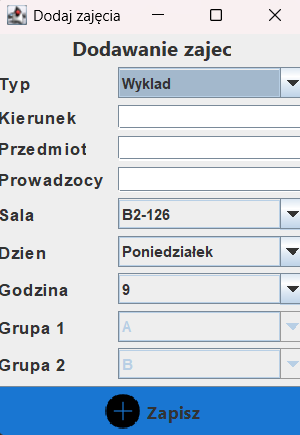
\includegraphics[width=0.45\textwidth]{figures/workApl/add_wyklad_panel.png}
\caption{Formularz dodawania zajęć typu Wykład}
\label{fig:add_wyklad}
\end{figure}

Użytkownik wprowadza dane dotyczące wykładu: kierunek, przedmiot, prowadzący, sala, dzień tygodnia, godzina. Zajęcia typu wykład są przypisane do wszystkich grup, więc pola \texttt{Grupa 1} i \texttt{Grupa 2} są wyszarzone.

\section*{Formularz dodawania zajęć typu Laboratorium}
\begin{figure}[H]
\centering
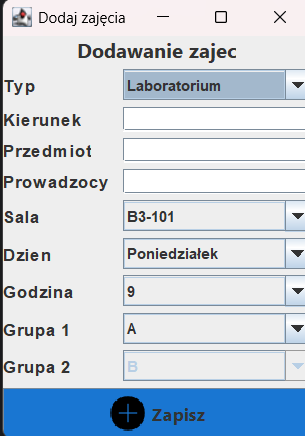
\includegraphics[width=0.45\textwidth]{figures/workApl/add_lab_panel.png}
\caption{Formularz dodawania zajęć typu Laboratorium}
\label{fig:add_lab}
\end{figure}

W tym formularzu użytkownik wybiera jedną grupę laboratoryjną, dla której są przeznaczone dane zajęcia. Pole \texttt{Grupa 2} jest wyłączone.

\section*{Formularz dodawania zajęć typu Projekt}
\begin{figure}[H]
\centering
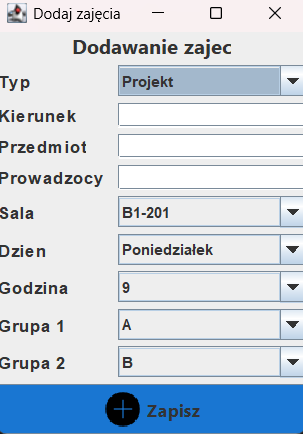
\includegraphics[width=0.45\textwidth]{figures/workApl/add_projekt_panel.png}
\caption{Formularz dodawania zajęć typu Projekt}
\label{fig:add_projekt}
\end{figure}

Dla zajęć typu Projekt dostępne są dwa pola wyboru grup: \texttt{Grupa 1} i \texttt{Grupa 2}. System wymusza wybranie obu, ponieważ projekty realizowane są wspólnie przez dwie grupy.

\section*{Formularz edycji zajęć}
\begin{figure}[H]
\centering
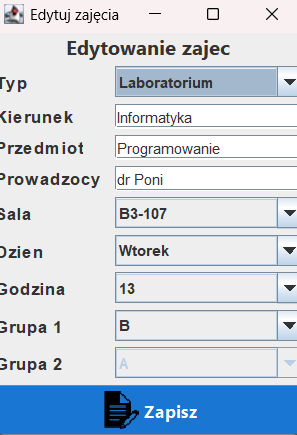
\includegraphics[width=0.45\textwidth]{figures/workApl/edit_panel.png}
\caption{Formularz edycji istniejących zajęć}
\label{fig:edit_panel}
\end{figure}

Formularz edycji pozwala na modyfikację danych wcześniej zapisanych zajęć. Po zaznaczeniu wiersza w tabeli, dane są automatycznie ładowane do formularza. Po kliknięciu \textbf{Zapisz}, rekord zostaje zaktualizowany w bazie danych. System waliduje dane przed zapisem.

